\chapter{Задание \textnumero1}

В листинге~\ref{lst:task01} приведён текст первой программы.

\begin{lstlisting}[label=lst:task01,caption={Текст первой программы}]
#include <stdio.h>
#include <fcntl.h>
#include <errno.h>
#include <unistd.h>
#include <stdlib.h>
#include <string.h>

int main(void)
{
    char c;
    char buff1[20];
    char buff2[20];
    int flag1, flag2;

    int fd = open("alphabet.txt", O_RDONLY);
    if (fd == -1)
    {
        fprintf(stderr, "%s: %s\n", "open alphabet.txt", strerror(errno));
        exit(1);
    }

    FILE *fs1 = fdopen(fd, "r");
    if (!fs1)
    {
        fprintf(stderr, "first fdopen %d: %s\n", fd, strerror(errno));
        exit(1);
    }
    setvbuf(fs1, buff1, _IOFBF, 20);
    FILE *fs2 = fdopen(fd, "r");
    if (!fs2)
    {
        fprintf(stderr, "second fdopen %d: %s\n", fd, strerror(errno));
        exit(1);
    }
    setvbuf(fs2, buff2, _IOFBF, 20);

    flag1 = flag2 = 1;
    while(flag1 == 1 || flag2 == 1)
    {
        flag1 = fscanf(fs1, "%c", &c);
        if (flag1 == 1)
            fprintf(stdout, "%c", c);

        flag2 = fscanf(fs2, "%c", &c);
        if (flag2 == 1)
            fprintf(stdout, "%c", c);
    }

    close(fd);

    return 0;
}

\end{lstlisting}

На рисунке~\ref{img:task01} изображён результат работы этой программы.

\begin{figure}[H]
    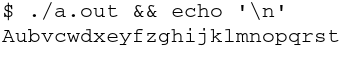
\includegraphics[scale=0.5]{images/task01}
    \caption{Результат работы первой программы}\label{img:task01}
\end{figure}

В рассматриваемой программе в результате вызова системного вызова open создается новый дескриптор файла, который открывается только на чтение. Так же создается запись в системной таблице открытых файлов. Текущая позиция устанавливается на начало файла.

Далее функция fdopen в результате двух вызовов создает два разных объекта структуры FILE~--- два потока ввода, ссылающихся на один ранее созданный файловый дескриптор, а функция setvbuf устанавливает блочную буферизацию размером 20 байт для этих потоков.

При первом вызове fscanf, то есть при первой операции чтения из файла, происходит заполнения буфера содержимым файла до тех пор, пока в нем есть место или пока не будет достигнут конец файла. Так как оба потока ссылаются на один и тот же файловый дескриптор (а значит и на одну и ту же запись в системной таблице открытых файлов) и размер каждого буфера равен 20 байт, то в первый в порядке чтения буфер будет записано первые 20 символов файла, в во второй~--- оставшиеся 6.

Таким образом, на экран выводится строка, состоящая из символов, поочередно выведенных из первого и из второго буферов.

На рисунке~\ref{pdf:task01} изображена связь между созданными дескрипторами.

\begin{figure}[H]
    \centering
    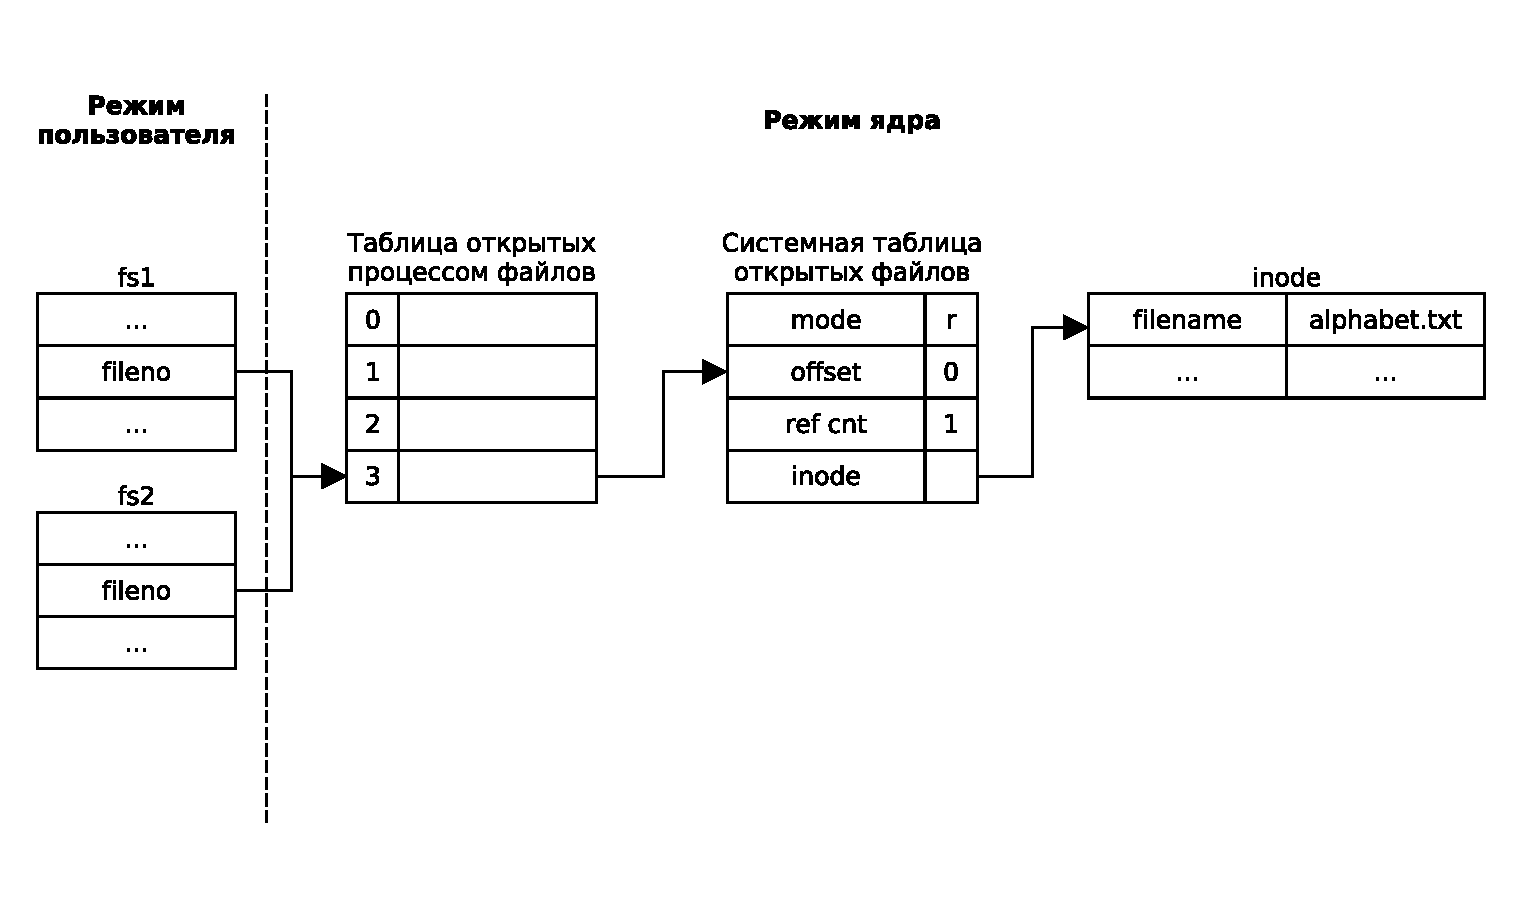
\includegraphics[scale=0.6]{pdf/task01.pdf}
    \caption{Связь между дескрипторами}\label{pdf:task01}
\end{figure}

